\documentclass[12pt]{article}
\usepackage[margin=1.5cm]{geometry}
\usepackage{amsmath}
\usepackage{graphicx}
\title{RC Circuits Lab: Electronic Filters}

\begin{document}
\maketitle

\section{Review: Two RC Circuits}

\begin{figure}
\centering
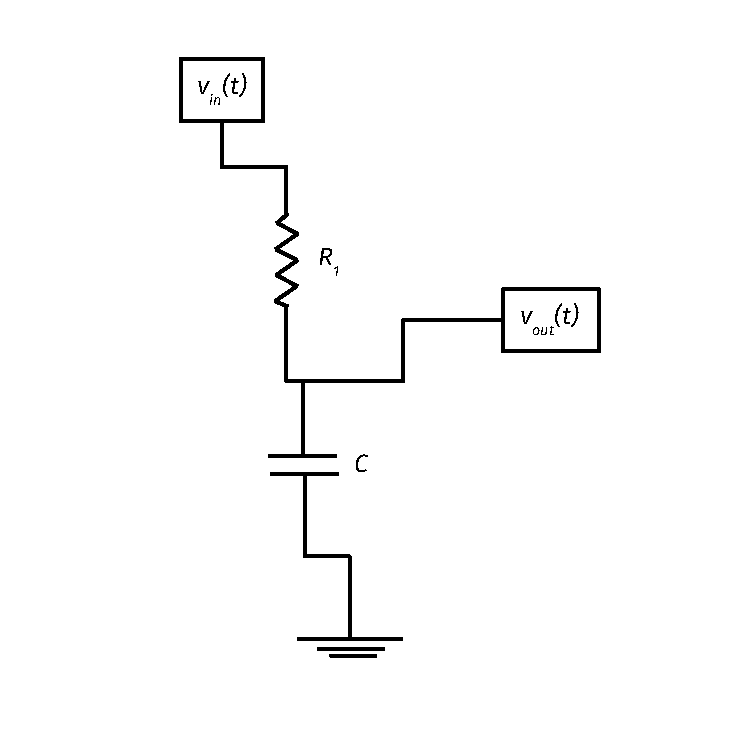
\includegraphics[width=0.35\textwidth,trim=0cm 1cm 0cm 0cm,clip=true]{LowPass.pdf}
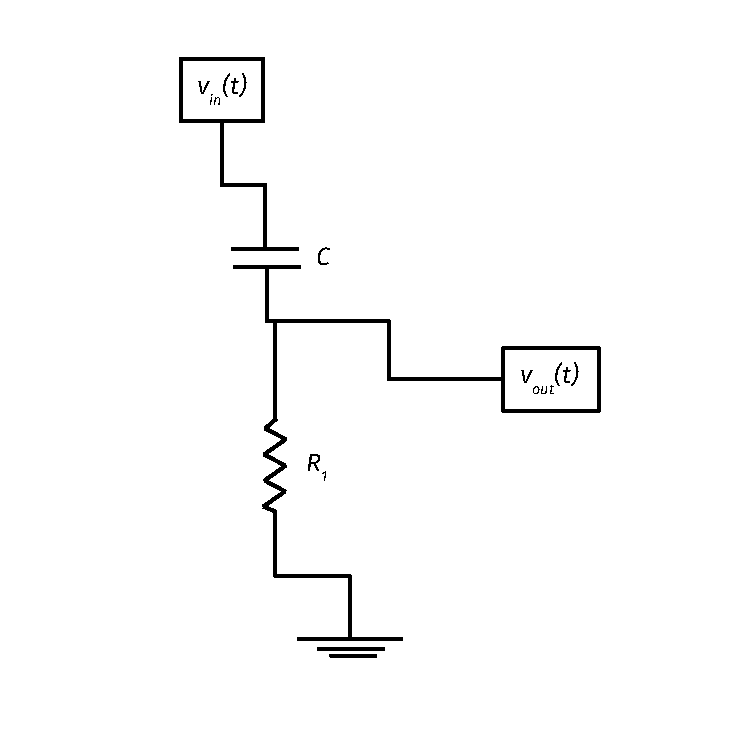
\includegraphics[width=0.35\textwidth,trim=0cm 1cm 0cm 0cm,clip=true]{HighPass.pdf}
\caption{\label{fig:fig2} (Left) A single-pole RC low-pass filter. (Right) A single-pole RC high-pass filter.}
\end{figure}

The \textbf{transfer function} of the RC circuit in Fig. \ref{fig:fig2} is the ratio of the output voltage to the input voltage, as with a voltage divider.  However, the derivation of this ratio produces

\begin{equation}
\frac{\tilde{v}_{out}(\omega)}{\tilde{v}_{in}(\omega)} = \frac{\frac{1}{j\omega C}}{R+\frac{1}{j\omega C}} = \frac{1}{j\omega R C + 1}
\label{eq:trans2}
\end{equation}

Let the \textit{time-constant} be defined as $\tau = RC$, and $\omega_0 = 1/\tau$.  Equation \ref{eq:trans2} may be written:

\begin{equation}
\frac{\tilde{v}_{out}(\omega)}{\tilde{v}_{in}(\omega)} = -\frac{j\omega_0}{\omega - j\omega_0}
\label{eq:eq6}
\end{equation}

The magnitude and phase of Eq. \ref{eq:eq6} are

\begin{align}
M_{LP}(\omega) &= \left( 1 + \left( \frac{\omega}{\omega_0}\right)^2 \right)^{-1/2} \\
\phi_{LP}(\omega) &= -\tan^{-1}\left(\frac{\omega}{\omega_0}\right)
\label{eq:eq7}
\end{align}

The low-pass transfer function $M_{LP}(\omega)$ attenuates frequencies much larger than $\omega_0$, and the $\phi_{LP}(\omega)$ function shows that there is a frequency-dependent phase-shift.  The high-pass filter in Fig. \ref{fig:fig2} (right) is similar to the low-pass filter in Fig. \ref{fig:fig2} (left).  Following the same arguments as the low-pass case, the complex transfer function is

\begin{equation}
\frac{\tilde{v}_{out}(\omega)}{\tilde{v}_{in}(\omega)} = \frac{\omega}{\omega - j\omega_0}
\label{eq:trans3}
\end{equation}

The magnitude and phase of Eq. \ref{eq:trans3} are

\begin{align}
M_{HP}(\omega) &= \left( 1 + \left( \frac{\omega_0}{\omega}\right)^2 \right)^{-1/2} \\
\phi_{HP}(\omega) &= \tan^{-1}\left(\frac{\omega_0}{\omega}\right)
\end{align}

Unlike the voltage divider, the circuits in Fig. \ref{fig:fig2} have capacitors.  The filtering in these cases is driven by how quickly these capacitors can be charged and discharged, regardless of where they are in the circuit.

\section{Building a Passive Differentiator}

Using the bread-board, wires, resistors, and capacitors, build a single-pole high-pass filter.  If $\omega \ll \omega_0$, the transfer function is approximately:

\begin{equation}
\frac{\tilde{v}_{out}(\omega)}{\tilde{v}_{in}(\omega)} \approx \frac{\omega}{-j\omega_0} = j\omega \tau = j\omega RC
\label{eq:eq19}
\end{equation}

Rearranging Eq. \ref{eq:eq19} and switching to the time-domain reveals the relationship between $v_{in}$ and $v_{out}$:

\begin{equation}
v_{out}(t) \approx \tau \frac{dv_{in}}{dt}
\label{eq:eq20}
\end{equation}

Equation \ref{eq:eq20} shows that for some frequencies, the circuit output is the derivative of the input, with a \textit{gain} equal to $\tau = RC$.  Choose a \textit{triangle wave} on the function generator, and draw the \textit{unfiltered} signal below on the left. Choose voltage as the y-axis, and time as the x-axis.  Make sure to record the units and scale of the axes.  For example, if the amplitude of the signal is 2.0 V, indicate that on the graph. On the right, draw the \textit{filtered signal.}

\begin{figure}[ht]
\centering
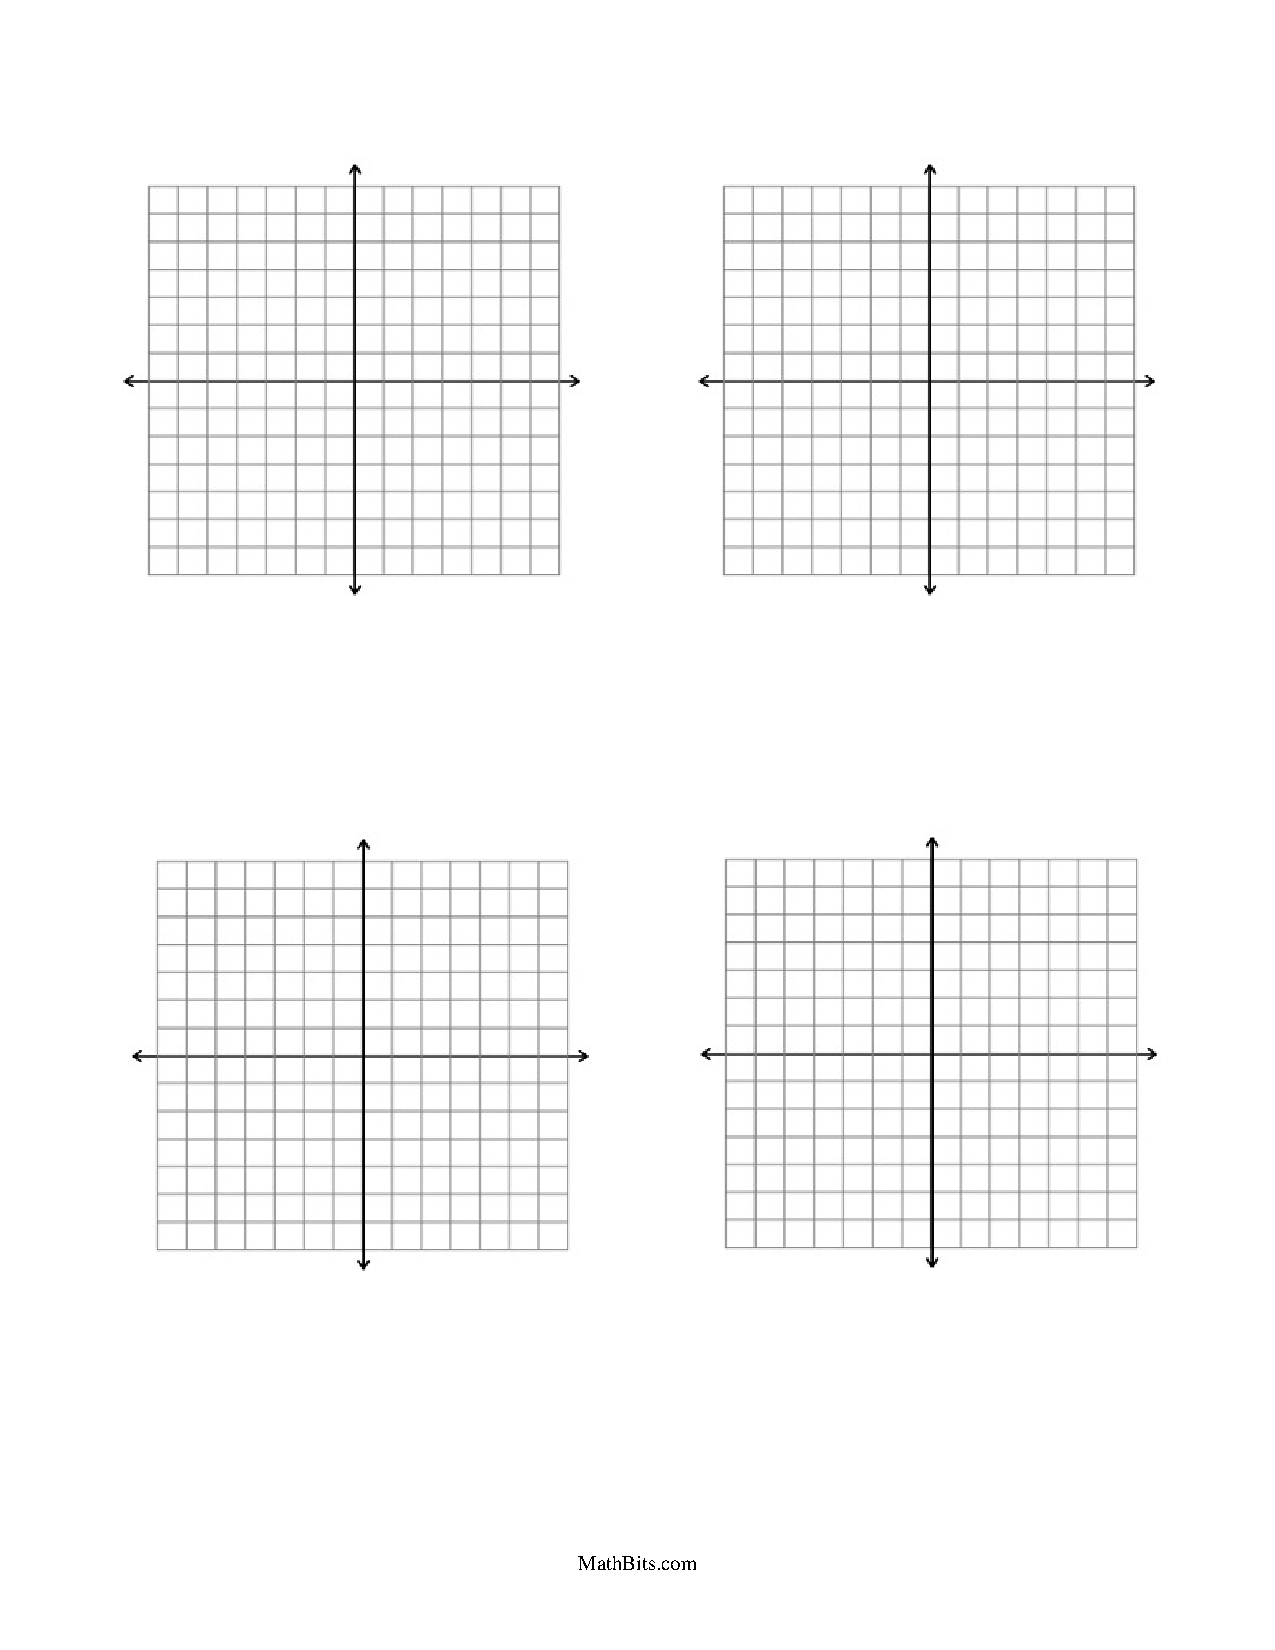
\includegraphics[width=0.9\textwidth,trim=0cm 18cm 0cm 2cm,clip=true]{axes.pdf}
\caption{\label{fig:axes} Plot your differentiator results here. Make sure to label your axes in scale and units.}
\end{figure}

\vspace{5cm}

\textbf{Questions:}
\begin{enumerate}
\item Explain the shape of the \textit{filtered} signal relative to the \textit{unfiltered} signal. What should the derivative of the triangle wave be? \\ \vspace{1.5cm}
\item What is the \textit{gain} of your filtered signal?  It should be a number close to the time constant of your circuit. Is the gain positive or negative? \\ \vspace{1.5cm}
\end{enumerate}

\section{Building a Passive Integrator}

Using the bread-board, wires, resistors, and capacitors, build a single-pole low-pass filter.  If $\omega \gg \omega_0$, the transfer function is approximately:

\begin{equation}
\frac{\tilde{v}_{out}(\omega)}{\tilde{v}_{in}(\omega)} \approx \frac{-j\omega_0}{\omega}
\label{eq:eq21}
\end{equation}

Rearranging Eq. \ref{eq:eq21} and switching to the time-domain reveals the relationship between $v_{in}$ and $v_{out}$:

\begin{equation}
v_{out}(t) = \frac{1}{\tau} \int_{t_1}^{t_2} v_{in}(t) dt
\label{eq:eq22}
\end{equation}

Equation \ref{eq:eq22} shows that for some frequencies, the circuit output is the integral of the input, with a \textit{gain} equal to $1/\tau$.  Choose a \textit{square wave} on the function generator, and draw the \textit{unfiltered} signal below on the left. Choose voltage as the y-axis, and time as the x-axis.  Make sure to record the units and scale of the axes.  For example, if the amplitude of the signal is 2.0 V, indicate that on the graph. On the right, draw the \textit{filtered signal.}

\begin{figure}[ht]
\centering
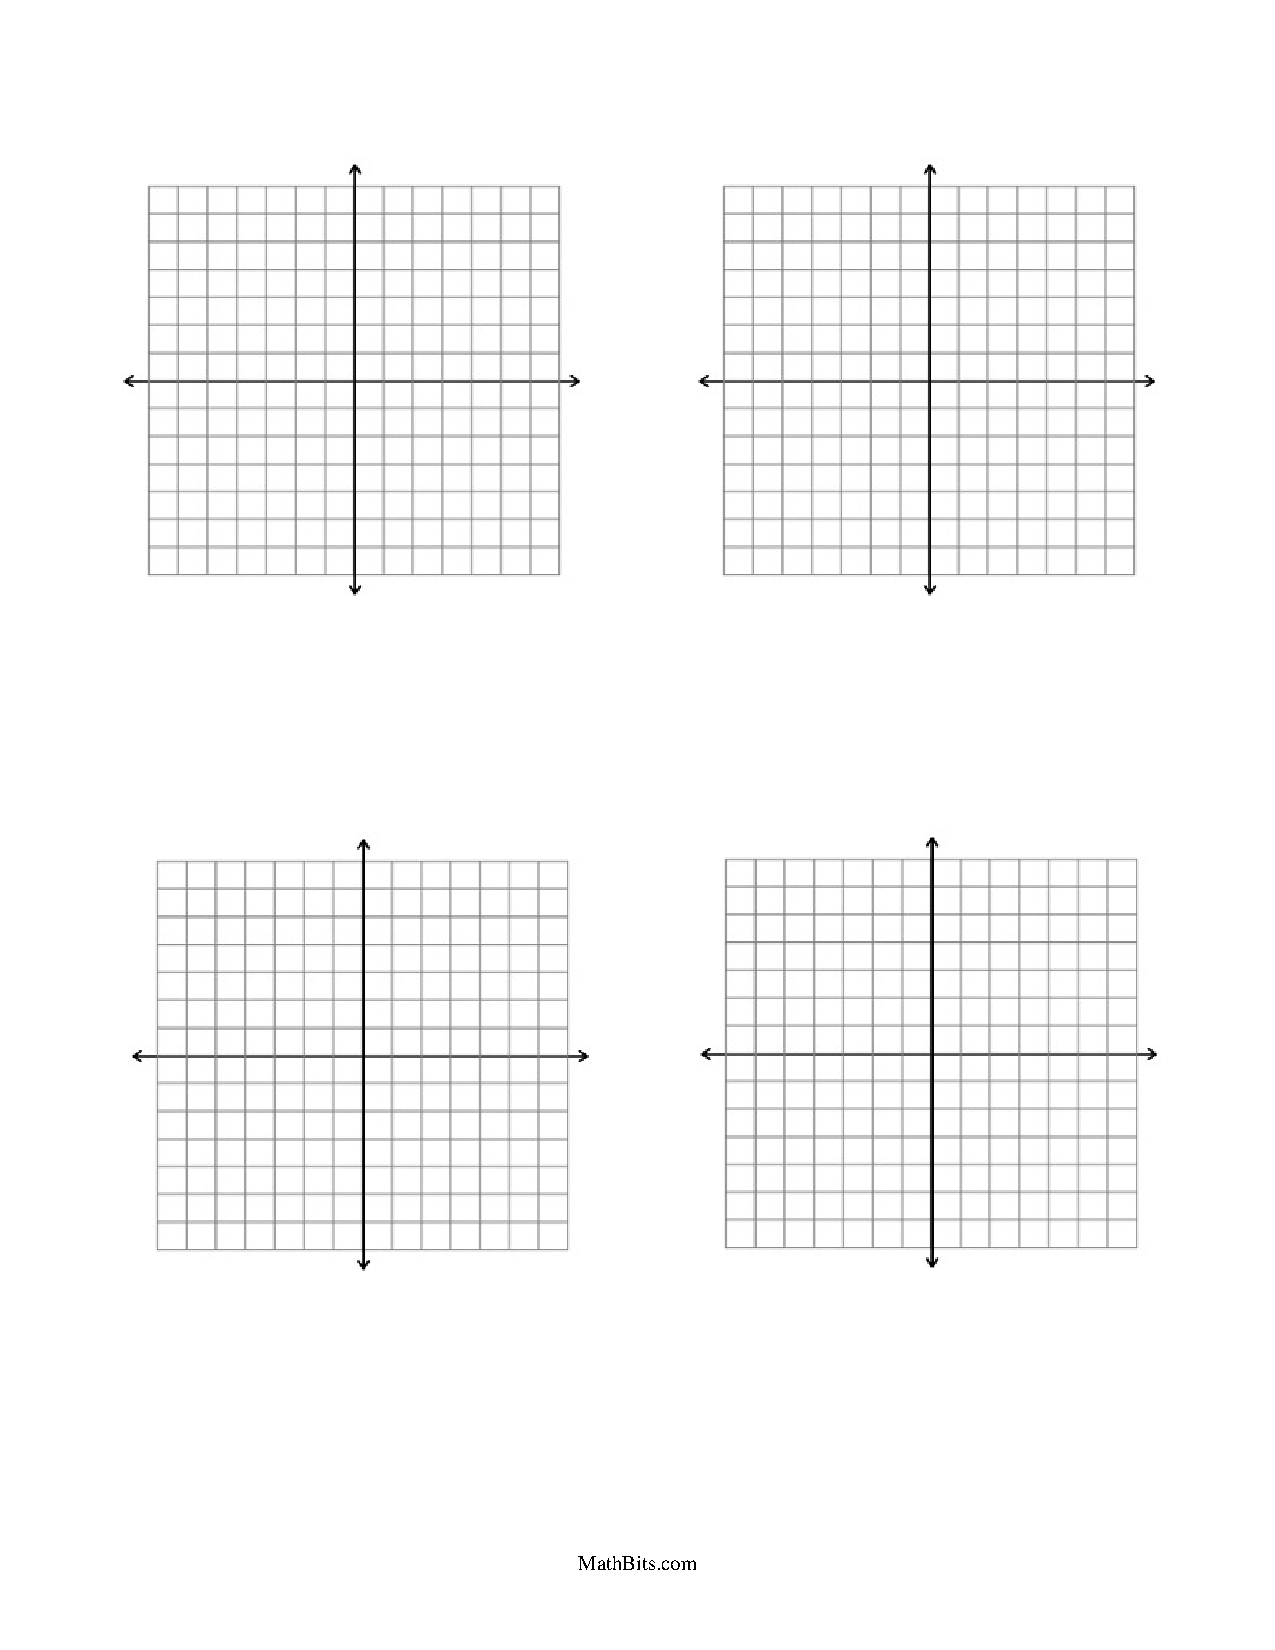
\includegraphics[width=0.9\textwidth,trim=0cm 18cm 0cm 2cm,clip=true]{axes.pdf}
\caption{\label{fig:axes} Plot your integrator results here. Make sure to label your axes in scale and units.}
\end{figure}

\vspace{5cm}

\textbf{Questions:}
\begin{enumerate}
\item Explain the shape of the \textit{filtered} signal relative to the \textit{unfiltered} signal. What should the integral of the square wave be? \\ \vspace{1.5cm}
\item What is the \textit{gain} of your filtered signal?  It should be a number close to the inverse of the time constant of your circuit. Is the gain positive or negative? \\ \vspace{1.5cm}
\end{enumerate}

\end{document}